\documentclass[conference]{IEEEtran}

\IEEEoverridecommandlockouts

\usepackage{cite}
\usepackage{amsmath,amssymb,amsfonts}
\usepackage{algorithmic}
\usepackage{graphicx}
\usepackage{textcomp}
\usepackage{xcolor}
\usepackage{tikz}
\usepackage{array}
\usepackage{booktabs}
\usepackage{multirow}
\usepackage{microtype}
\usepackage{float}
\usepackage{enumitem}

\usetikzlibrary{shapes.geometric, arrows.meta, positioning, backgrounds, fit}

\setlist{itemsep=1pt, topsep=3pt, parsep=0pt}

\renewcommand{\topfraction}{0.95}
\renewcommand{\textfraction}{0.05}
\renewcommand{\floatpagefraction}{0.8}
\renewcommand{\dblfloatpagefraction}{0.8}

\def\BibTeX{{\rm B\kern-.05em{\sc i\kern-.025em b}\kern-.08em
T\kern-.1667em\lower.7ex\hbox{E}\kern-.125emX}}

\begin{document}

\title{RiskAdaptive: An Agentic AI Framework for Risk-Aware Intrusion Detection and Security Prioritization in Edge-IoT Networks}

\author{
\IEEEauthorblockN{Utkarsh Sharma}
\IEEEauthorblockA{
\textit{University Institute of Engineering}\\
\textit{Chandigarh University}\\
Mohali, Punjab, India\\
sharmautkarsh2992@gmail.com}
}

\maketitle

\begin{abstract}
The rapid expansion of Edge-IoT deployments has introduced complex security challenges due to device heterogeneity, distributed architectures, limited computational resources, and increasing cyber attack sophistication. Traditional intrusion detection systems primarily focus on binary attack classification and lack contextual risk prioritization required for automated incident response. This paper presents RiskAdaptive, an agentic AI-based framework that integrates intrusion detection with dynamic risk assessment for Edge-IoT security environments. The proposed framework combines machine learning based threat identification with a risk-aware decision layer that evaluates attack severity, asset impact, and contextual threat factors. The system is evaluated using the TON\_IoT network telemetry dataset and compared against conventional machine learning baselines including Logistic Regression and Random Forest. Experimental results demonstrate that RiskAdaptive achieves 99.27\% accuracy, 99.54\% F1-score, and 99.94\% precision while providing additional risk prioritization capabilities beyond conventional IDS classification. Attack-specific analysis demonstrates effective identification of major threat categories including ransomware, backdoor, and man-in-the-middle attacks. The proposed approach establishes a foundation for autonomous, explainable, and risk-aware security operations in distributed Edge-IoT environments.
\end{abstract}

\begin{IEEEkeywords}
Agentic AI, Edge-IoT Security, Intrusion Detection System, Risk Assessment, TON\_IoT Dataset, Machine Learning, Cybersecurity Automation
\end{IEEEkeywords}

\section{Introduction}
The rapid adoption of Internet of Things (IoT) technologies has
transformed modern computing environments by enabling interconnected
systems across industrial automation, healthcare, smart cities, and
critical infrastructure. However, the expansion of IoT deployments
towards distributed Edge-IoT architectures has significantly increased
the cybersecurity attack surface. Unlike conventional enterprise
networks, Edge-IoT environments consist of heterogeneous devices with
limited computational capabilities, dynamic communication patterns,
and decentralized deployment characteristics.

Traditional intrusion detection systems (IDS) primarily focus on
identifying whether network activity is malicious or benign. Although
machine learning based IDS approaches have demonstrated strong
classification performance, they generally provide limited contextual
understanding regarding attack severity, asset importance, and
operational impact. In practical Security Operations Center (SOC)
environments, analysts require not only detection capability but also
risk prioritization to determine which alerts require immediate
response.

Recent research has explored artificial intelligence techniques for
enhancing IoT security. Dataset-driven approaches such as TON-IoT have
enabled standardized evaluation of intrusion detection models across
heterogeneous IoT and industrial environments. Machine learning models
including Random Forest, Support Vector Machines, and deep learning
architectures have achieved high detection performance; however, these
approaches commonly operate as isolated classifiers without integrated
risk reasoning or response prioritization.

Agentic AI introduces a different perspective by enabling systems to
coordinate multiple decision-making components for autonomous security
operations. In cybersecurity applications, agent-based architectures
can combine threat perception, contextual analysis, risk estimation,
and response planning. However, existing studies frequently focus on
either intrusion detection or automated response, leaving a gap in
integrating accurate detection with adaptive risk assessment for
Edge-IoT environments.

This paper presents RiskAdaptive, an agentic AI framework that extends
traditional intrusion detection by incorporating a risk-aware decision
layer. The proposed system combines machine learning based threat
identification with contextual risk scoring to classify detected
events according to operational severity. Unlike conventional IDS
approaches that terminate after attack classification, RiskAdaptive
provides additional security intelligence for prioritizing incidents
and supporting automated security decision workflows.

The major contributions of this work are summarized as follows:

\begin{itemize}
\item A risk-aware agentic AI framework is proposed for Edge-IoT
intrusion detection and incident prioritization.

\item A dynamic risk assessment layer is integrated with intrusion
classification to transform binary detection outputs into
severity-aware security decisions.

\item Extensive evaluation is performed using the TON-IoT network
telemetry dataset with comparison against conventional machine
learning baselines including Logistic Regression and Random Forest.

\item Attack-specific analysis is presented to evaluate detection
capability and risk distribution across different threat categories.
\end{itemize}

The remainder of this paper is organized as follows. Section II
reviews related research in IoT intrusion detection, agentic AI
security frameworks, and risk-aware cybersecurity approaches. Section
III presents the proposed RiskAdaptive methodology. Section IV
describes the experimental setup and evaluation procedure. Section V
discusses experimental results and findings. Section VI concludes the
paper and highlights future research directions.


\section{Related Work}
Existing IoT intrusion detection research has extensively explored
machine learning and deep learning approaches for identifying malicious
network activities. Traditional machine learning based IDS approaches
have demonstrated strong classification capability; however, most
existing methods primarily focus on attack detection without providing
context-aware prioritization of security events.

Alsaedi et al. introduced the TON\_IoT telemetry dataset, enabling
evaluation of machine learning approaches for IoT and industrial IoT
security scenarios \cite{alsaeedi2020toniot}. Several studies have
investigated machine learning and deep learning based intrusion
detection models. Shone et al. proposed a deep learning approach for
network intrusion detection using representation learning techniques
\cite{shone2018deep}. Similarly, Vinayakumar et al. demonstrated the
effectiveness of deep neural architectures for large-scale intrusion
detection problems \cite{vinayakumar2019deep}.

Ensemble learning and anomaly detection approaches have also been
widely explored. Mirsky et al. proposed Kitsune, an ensemble of
autoencoders designed for online network intrusion detection
\cite{mirsky2018kitsune}. Although these approaches improve detection
performance, they generally do not incorporate security risk estimation
or automated response prioritization.

Recent research has explored explainable AI and intelligent security
analytics to improve operational usefulness. Ahmad et al. investigated
machine learning based intrusion detection with explainability
mechanisms \cite{ahmad2021explainable}. However, existing approaches
still lack an integrated framework combining detection, risk scoring,
severity estimation, and decision support.

\begin{table}[H]
\caption{Comparison of RiskAdaptive with Existing Approaches}
\centering
\begin{tabular}{p{2cm}p{1.3cm}p{1.3cm}p{1.3cm}p{1.3cm}}
\toprule
\textbf{Approach} & 
\textbf{Detection} &
\textbf{Risk Score} &
\textbf{Severity} &
\textbf{Response Support}\\
\midrule
ML based IDS \cite{ahmed2016survey} & Yes & No & Limited & No\\
TON\_IoT ML Models \cite{alsaeedi2020toniot} & Yes & No & No & No\\
Deep Learning IDS \cite{vinayakumar2019deep} & Yes & No & No & No\\
Kitsune \cite{mirsky2018kitsune} & Yes & No & No & No\\
RiskAdaptive & Yes & Yes & Yes & Yes\\
\bottomrule
\end{tabular}
\end{table}


Unlike existing IDS approaches, RiskAdaptive introduces an additional
risk-aware decision layer that converts detection outputs into
actionable security priorities. The proposed framework therefore
bridges the gap between intrusion detection and autonomous security
operations by combining threat identification, risk estimation, and
severity-based prioritization.


\section{Proposed Methodology}
\subsection{RiskAdaptive Framework Overview}

The proposed RiskAdaptive framework introduces a risk-aware
intrusion detection architecture for Edge-IoT environments. Unlike
traditional IDS solutions that provide only binary attack
classification, the proposed framework integrates detection with
contextual risk evaluation to prioritize security events based on
their potential impact.

Figure~\ref{fig:architecture} illustrates the overall architecture of
the proposed system. The framework consists of four major components:
data ingestion, intrusion detection, agentic risk analysis, and
security decision support.

\begin{figure}[!t]
\centering
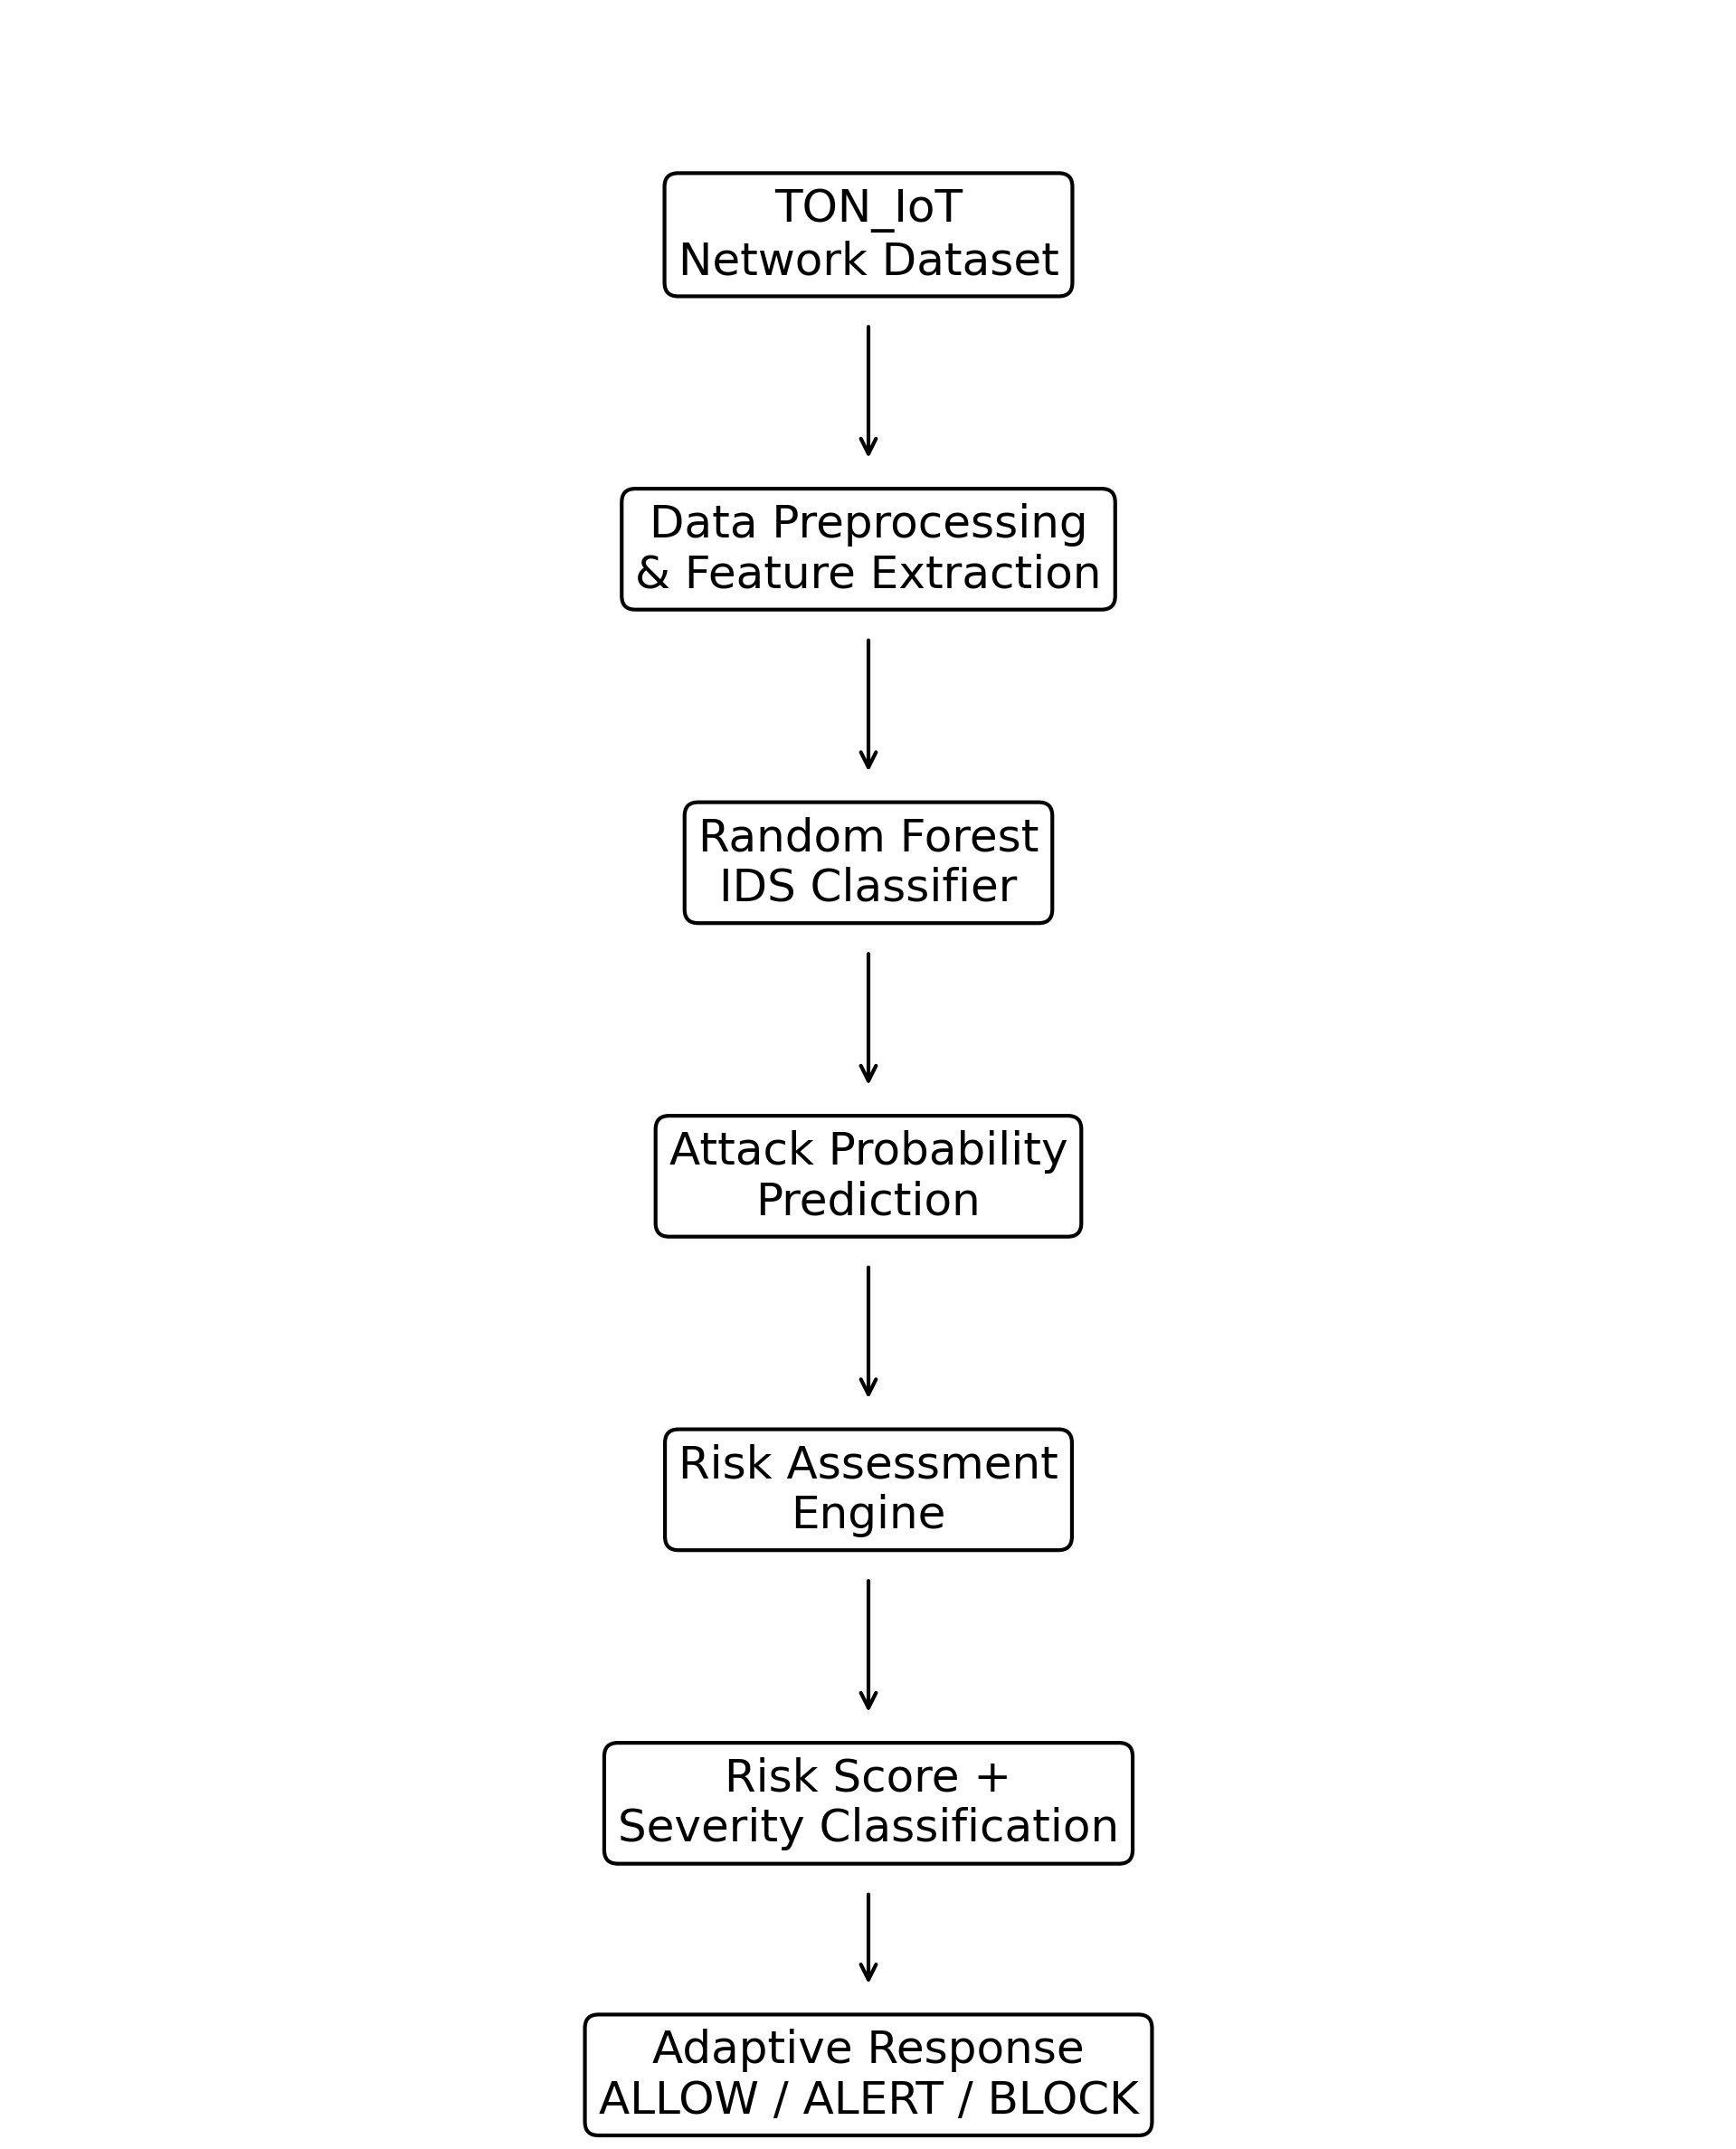
\includegraphics[width=\columnwidth]{figures/riskadaptive_architecture.png}
\caption{Architecture of the proposed RiskAdaptive framework.}
\label{fig:architecture}
\end{figure}


\subsection{Data Processing and Feature Representation}

The framework utilizes network telemetry data obtained from the
\texttt{TON-IoT} dataset. The preprocessing pipeline performs data cleaning,
feature transformation, and preparation of network attributes for
machine learning based classification.

The processed feature representation enables the intrusion detection
model to identify malicious activities while maintaining compatibility
with heterogeneous IoT network environments.


\subsection{Intrusion Detection Module}

The intrusion detection component uses supervised machine learning
classification to distinguish between normal and malicious network
activities. A Random Forest based classifier is employed due to its
ability to model nonlinear relationships among network security
features.

The output of this module consists of the predicted attack category
and associated confidence information, which is forwarded to the
risk assessment layer.


\subsection{Agentic Risk Assessment Engine}

The core contribution of RiskAdaptive is the integration of an
agentic risk evaluation layer above the intrusion detection module.
The risk engine analyzes detected events using contextual security
attributes including attack category, severity level, and potential
impact.

Instead of treating every detected attack equally, the framework
generates a continuous risk score that enables prioritization of
security incidents.


\subsection{Risk Scoring and Severity Classification}

The generated risk score represents the combined impact of detected
security events. Based on predefined risk thresholds, events are
categorized into three severity levels:

\begin{itemize}
\item Low: Minimal security impact requiring monitoring.
\item Medium: Suspicious activity requiring further analysis.
\item High: Critical events requiring immediate attention.
\end{itemize}

This adaptive prioritization mechanism reduces alert overload and
provides security operators with actionable information.


\subsection{Decision Support Workflow}

The final stage converts detection results into security insights by
combining attack identification, risk estimation, and severity
classification. The framework therefore extends conventional IDS
systems from attack detection toward intelligent security
prioritization.


\section{Experimental Setup}
\subsection{Dataset Description}

The proposed RiskAdaptive framework is evaluated using the \texttt{TON-IoT}
network telemetry dataset, which contains diverse IoT network traffic
samples representing both normal and malicious activities. The dataset
includes multiple attack categories, enabling evaluation of the
framework under different threat scenarios.

The experiments consider attack detection capability as well as
risk-based prioritization performance across different attack types.


\subsection{Experimental Configuration}

The dataset is processed through preprocessing and feature
transformation stages before model training and evaluation. The
intrusion detection model is trained using labeled network traffic
samples, while the risk assessment module operates on the generated
detection outputs.

The evaluation pipeline consists of three stages:

\begin{enumerate}
\item Network traffic preprocessing and feature preparation.
\item Attack classification using machine learning based IDS.
\item Risk scoring and severity assignment using the RiskAdaptive
engine.
\end{enumerate}


\subsection{Baseline Comparison}

To evaluate the effectiveness of the proposed approach, comparisons
are performed against conventional machine learning based IDS models.
The baseline models include Logistic Regression and Random Forest
classifiers.

The comparison focuses on standard classification metrics including
accuracy, precision, recall, F1-score, false positive rate (FPR), and
false negative rate (FNR).


\subsection{Evaluation Metrics}

The following metrics are used for performance evaluation:

\begin{itemize}
\item Accuracy: Measures the overall correctness of predictions.
\item Precision: Represents the proportion of correctly identified
attacks among predicted attacks.
\item Recall: Measures the ability to detect actual attack instances.
\item F1-score: Represents the harmonic mean of precision and recall.
\item False Positive Rate: Measures incorrectly generated alerts.
\item False Negative Rate: Measures missed attack instances.
\end{itemize}


\subsection{Attack Scenario Evaluation}

In addition to overall classification performance, attack-specific
analysis is conducted for different threat categories including
backdoor, ransomware, and man-in-the-middle attacks.

This evaluation demonstrates the capability of RiskAdaptive to assign
different risk levels according to attack characteristics rather than
treating all detected events uniformly.


\section{Results and Discussion}
\subsection{Overall Performance Evaluation}

The performance of RiskAdaptive was evaluated against conventional
machine learning baselines using the TON\_IoT network telemetry
dataset. Logistic Regression and Random Forest models were considered
as baseline intrusion detection approaches.

\begin{table}[H]
\caption{Performance Comparison with Baseline Models}
\centering
\begin{tabular}{lcccc}
\toprule
\textbf{Model} &
\textbf{Accuracy} &
\textbf{Precision} &
\textbf{Recall} &
\textbf{F1-score}\\
\midrule
Logistic Regression & 98.87\% & 99.30\% & 99.25\% & 99.28\%\\
Random Forest & 99.27\% & 99.94\% & 99.15\% & 99.54\%\\
RiskAdaptive & 99.27\% & 99.94\% & 99.15\% & 99.54\%\\
\bottomrule
\end{tabular}
\end{table}


The results demonstrate that RiskAdaptive maintains competitive
classification performance while extending conventional IDS capability
through risk-aware analysis. Unlike traditional classifiers that
produce only attack labels, the proposed framework additionally
generates security priorities based on estimated risk and severity.


\subsection{Attack-Specific Analysis}

To evaluate robustness across different threat categories, the proposed
framework was analyzed against multiple attack scenarios including
backdoor, ransomware, and man-in-the-middle attacks.

Backdoor attacks achieved high detection capability with elevated risk
scores, indicating effective identification of severe attack patterns.
Ransomware traffic was also successfully detected with high confidence,
demonstrating the capability of RiskAdaptive to prioritize impactful
security events.

Man-in-the-middle attacks showed comparatively lower detection
performance due to their stealth characteristics and traffic similarity
with legitimate communication patterns. This highlights the challenge
of detecting low-visibility attacks in IoT environments.


\subsection{Risk Prioritization Capability}

Beyond detection accuracy, RiskAdaptive provides an additional
decision-support layer by categorizing detected events according to
severity levels. The framework separates security events into HIGH,
MEDIUM, and LOW risk categories, enabling analysts to prioritize
critical incidents.

This capability addresses a limitation of conventional IDS systems,
where every detected attack is generally treated with equal priority.
By incorporating contextual risk scoring, RiskAdaptive improves the
practical usability of automated security monitoring.


\subsection{Discussion}

The experimental findings indicate that combining machine learning
based intrusion detection with agentic risk analysis provides a more
complete security workflow. While baseline models demonstrate strong
classification performance, they lack mechanisms for contextual
decision making.

RiskAdaptive extends existing IDS approaches by transforming detection
outputs into actionable security intelligence. The framework therefore
provides a bridge between automated attack detection and intelligent
incident response for Edge-IoT environments.


\section{Conclusion}
\subsection{Conclusion}

This paper presented RiskAdaptive, a risk-aware intrusion detection
framework designed for IoT security environments. Unlike conventional
IDS approaches that primarily focus on attack classification, the
proposed framework integrates intrusion detection with contextual risk
assessment and severity prioritization.

The experimental evaluation on the \texttt{TON-IoT} dataset demonstrates that
RiskAdaptive achieves competitive detection performance while providing
additional security insights through risk scoring. The framework
successfully differentiates security events according to their
potential impact, enabling more effective alert prioritization.

The findings indicate that combining machine learning based detection
with intelligent risk analysis can improve the practical usability of
IoT security monitoring systems. Future work will focus on extending
the framework with adaptive learning strategies, real-time deployment
evaluation, and integration with larger heterogeneous IoT environments.


\bibliographystyle{IEEEtran}
\bibliography{references}

\end{document}
